%%%%%%%%%%%%%%%%%%%%%%%%%%%%%%%%%%%%%%%%%%%%%%%%%%%%%%%%%%%%%%%%%%%%%%%%%%%%%%%

\chapter{CONVOLUÇÃO}

A convolução é uma operação algébrica sobre duas funções que produz uma terceira função como resultado. Por função subentende-se funções contínuas ou sinais discretos. Para duas funções contínuas $x(t)$ e $y(t)$, a convolução destas é $z(t) = x(t) \star y(t)$ e é assim definida \cite{paris2001convolution}:

\begin{equation}
z(t) = \int_{-\infty}^{+\infty}x(\tau)y(t-\tau)d\tau.
\end{equation}

Essa integral existe para todos os valores de $t$, e o resultado $z(t)$ também é contínuo. A variável $\tau$ é simplesmente uma variável de integração e portanto não aparece no resultado. Essa variável aparece associada a $t$ no argumento de $y(t-\tau)$, indicando que essa função está deslocada no tempo com relação a $x(\tau)$ por um fator $t$ que também varia. Como ilustração, considere as funções abaixo:

\begin{equation}
x(t) = \exp\left(-\frac{t}{2}\right) u(t),
\label{eq:conv}
\end{equation}

\begin{equation*}
y(t) =  \left\{ \begin{array}{rl} 
\frac{t}{5}  & \text{para } 0 \leq t \leq 5,  \\
0 & \text{caso contrário}
\end{array}\right.
\end{equation*}

onde $u(t)=1$ para $t \geq 0$ e $u(t)=0$ caso contrário. As funções $x(t)$ e $y(t)$ são exibidas na Figura \ref{fig:1}, bem como a convolução destas $z(t)$. A partir da Eq. \ref{eq:conv}, a função $z(t)$ pode ser calculada com a integral do produto de $x(\tau)$ e $y(t-\tau)$, ou seja, de $x(\tau)$ com uma função $y$ que viaja da esquerda para a direita conforme $t$. A coluna da direita da Figura \ref{fig:2} ilustra o produto das respectivas funções na coluna da esquerda. A convolução é a integral do produto, isto é, a área indicada nos plots da coluna à direita. Conforme $t$ varia, a função $y$ translada da esquerda para a direita alterando o valor da integral. Novamente se verifica que o resultado da convolução depende de $t$, por isso $z(t)$.  

\begin{figure}[ht!]
	\caption{Funções do exemplo de convolução.}
	\vspace{1mm}	% acrescentar o espaçamento vertical apropriado entre o título e a borda superior da figura
	\begin{center}
		\resizebox{15cm}{!}{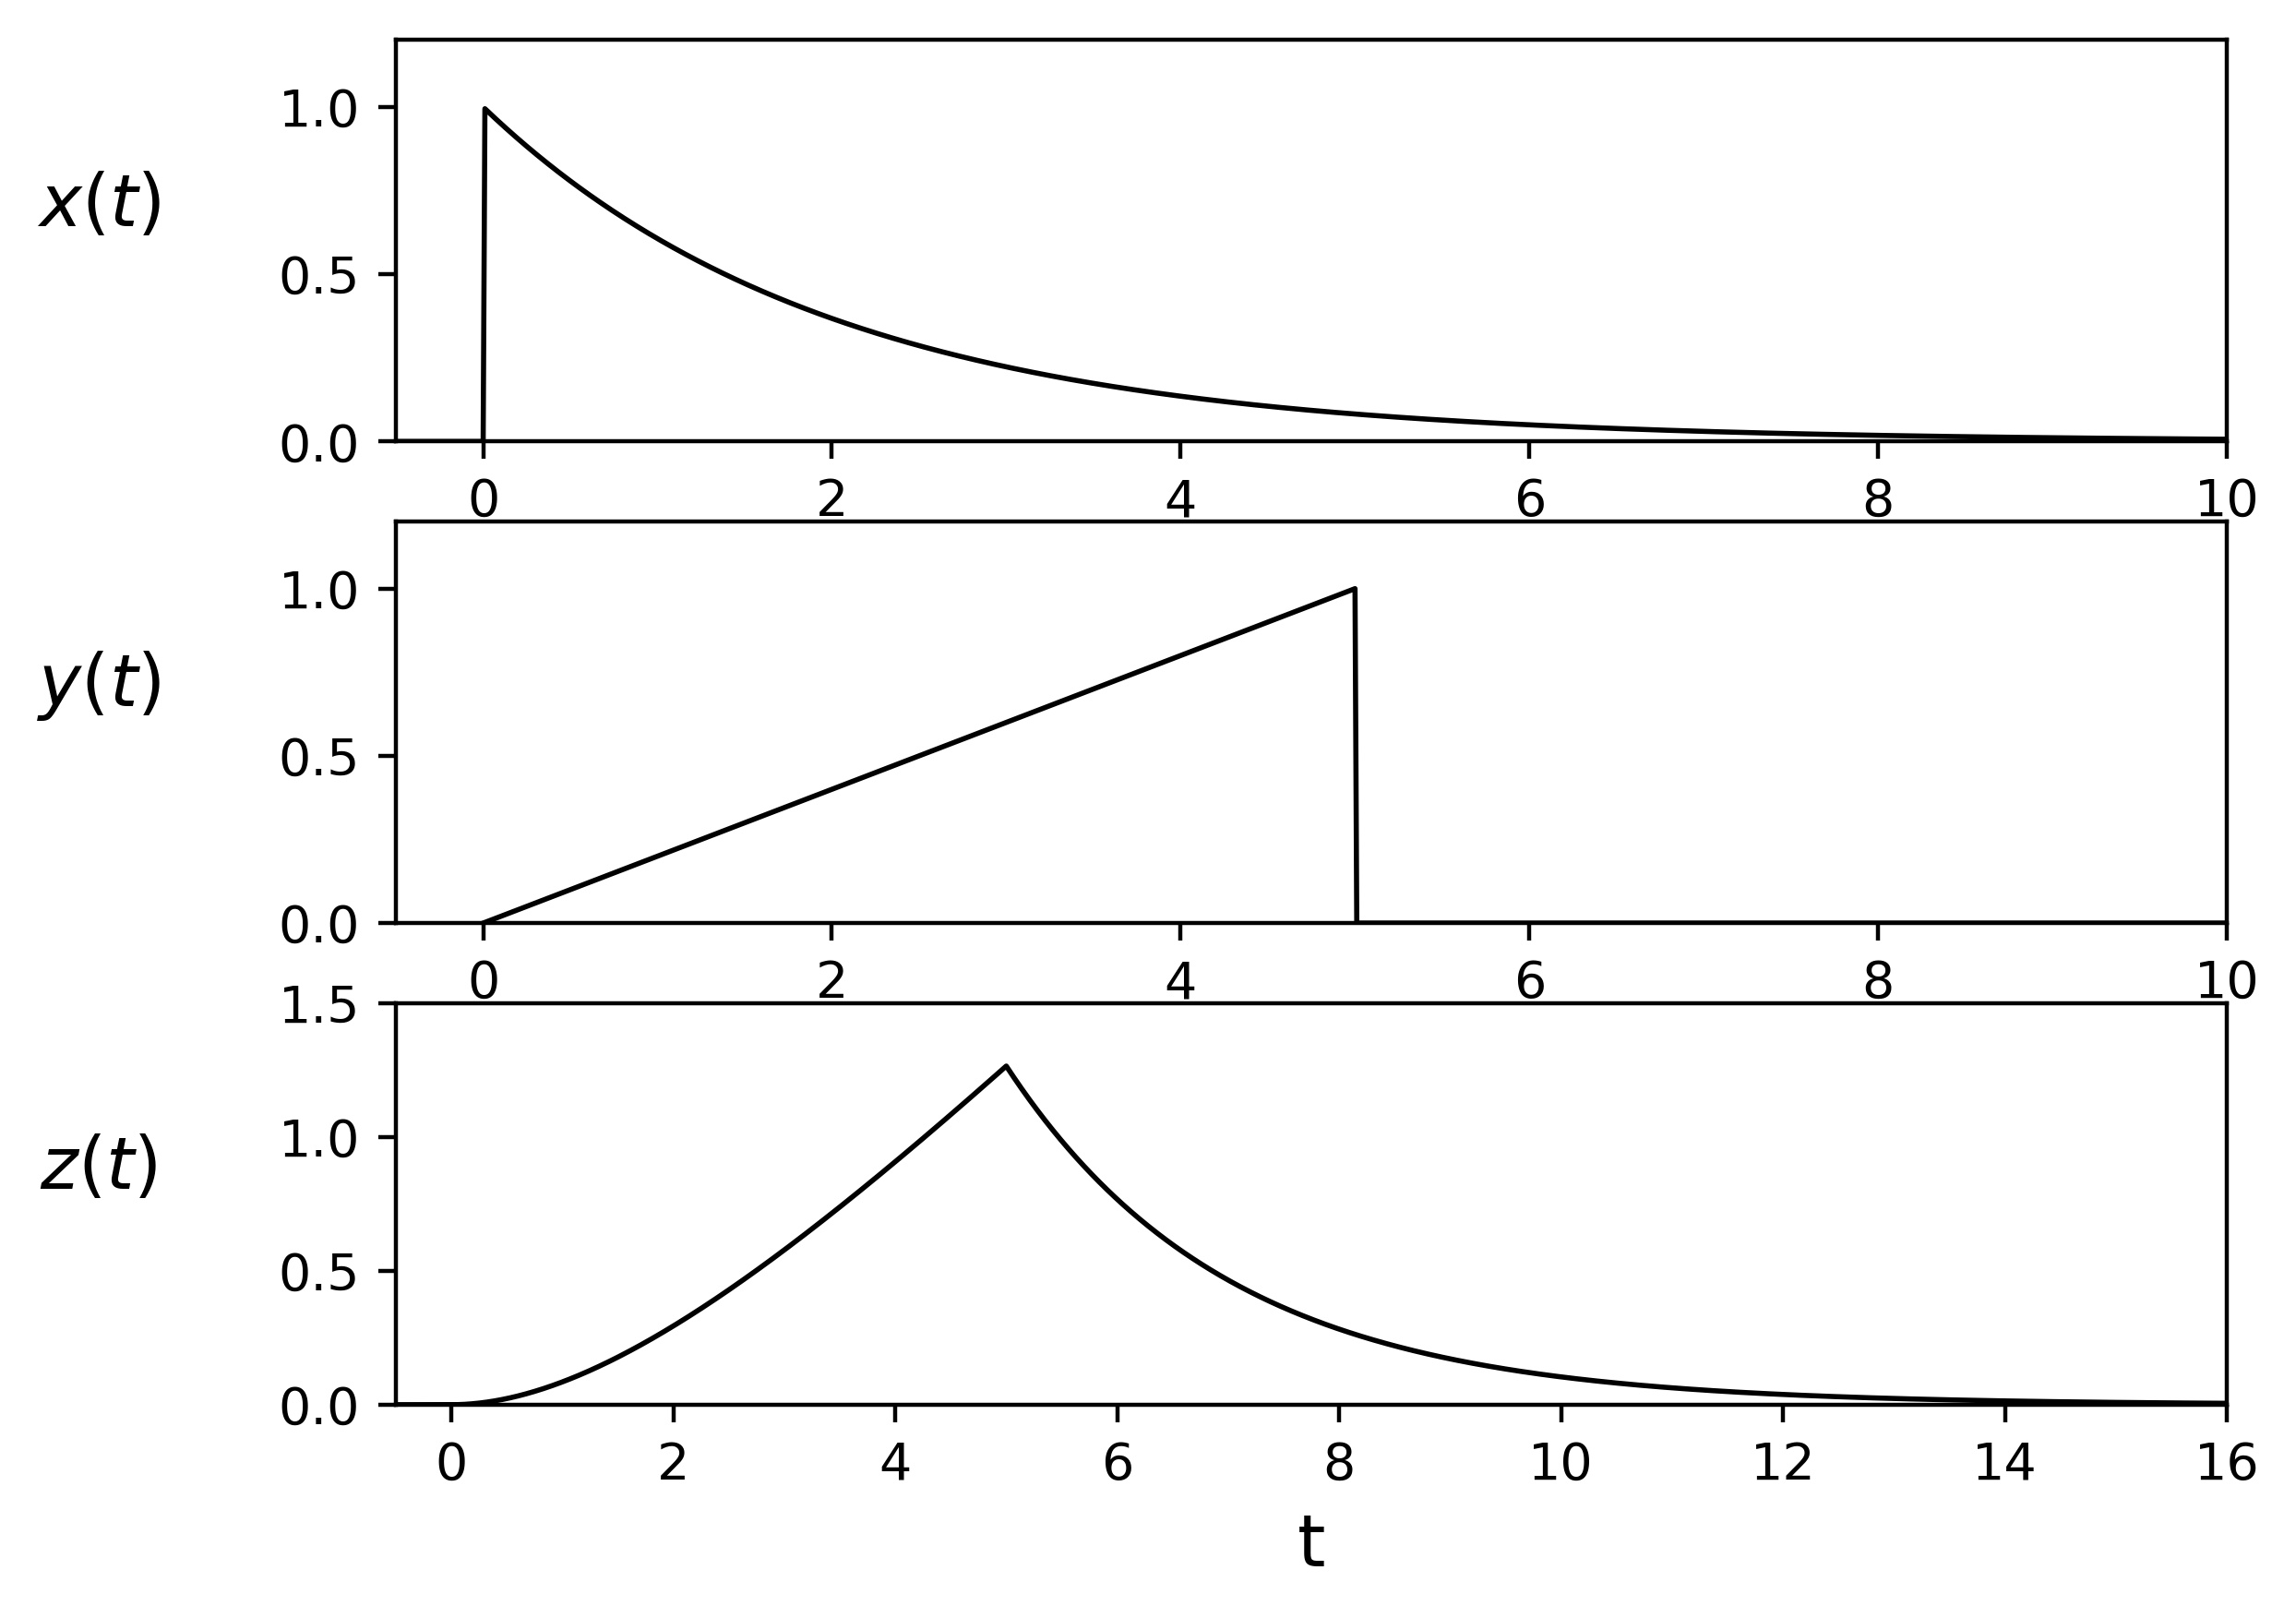
\includegraphics{Figuras/x_y.jpg}}
	\end{center}
	\vspace{1mm}	% acrescentar o espaçamento vertical apropriado entre a borda inferior da figura e a legenda ou a fonte quando não há legenda (o valor pode ser negativo para subir)
	\legenda{Topo: função $x(t)$; meio: função $y(t)$; abaixo: a convolução destas, $z(t)$.}	% legenda - para deixar sem legenda usar comando \legenda{} (nunca deve-se comentar o comando \legenda)
	\label{fig:1}
	%\FONTE{\url{https://omniweb.gsfc.nasa.gov/form/dx1.html}.}	% fonte consultada (elemento obrigatório, mesmo que seja produção do próprio autor)
\end{figure}

\begin{figure}[ht!]
	\caption{Convolução de duas funções.}
	\vspace{1mm}	% acrescentar o espaçamento vertical apropriado entre o título e a borda superior da figura
	\begin{center}
		\resizebox{15cm}{!}{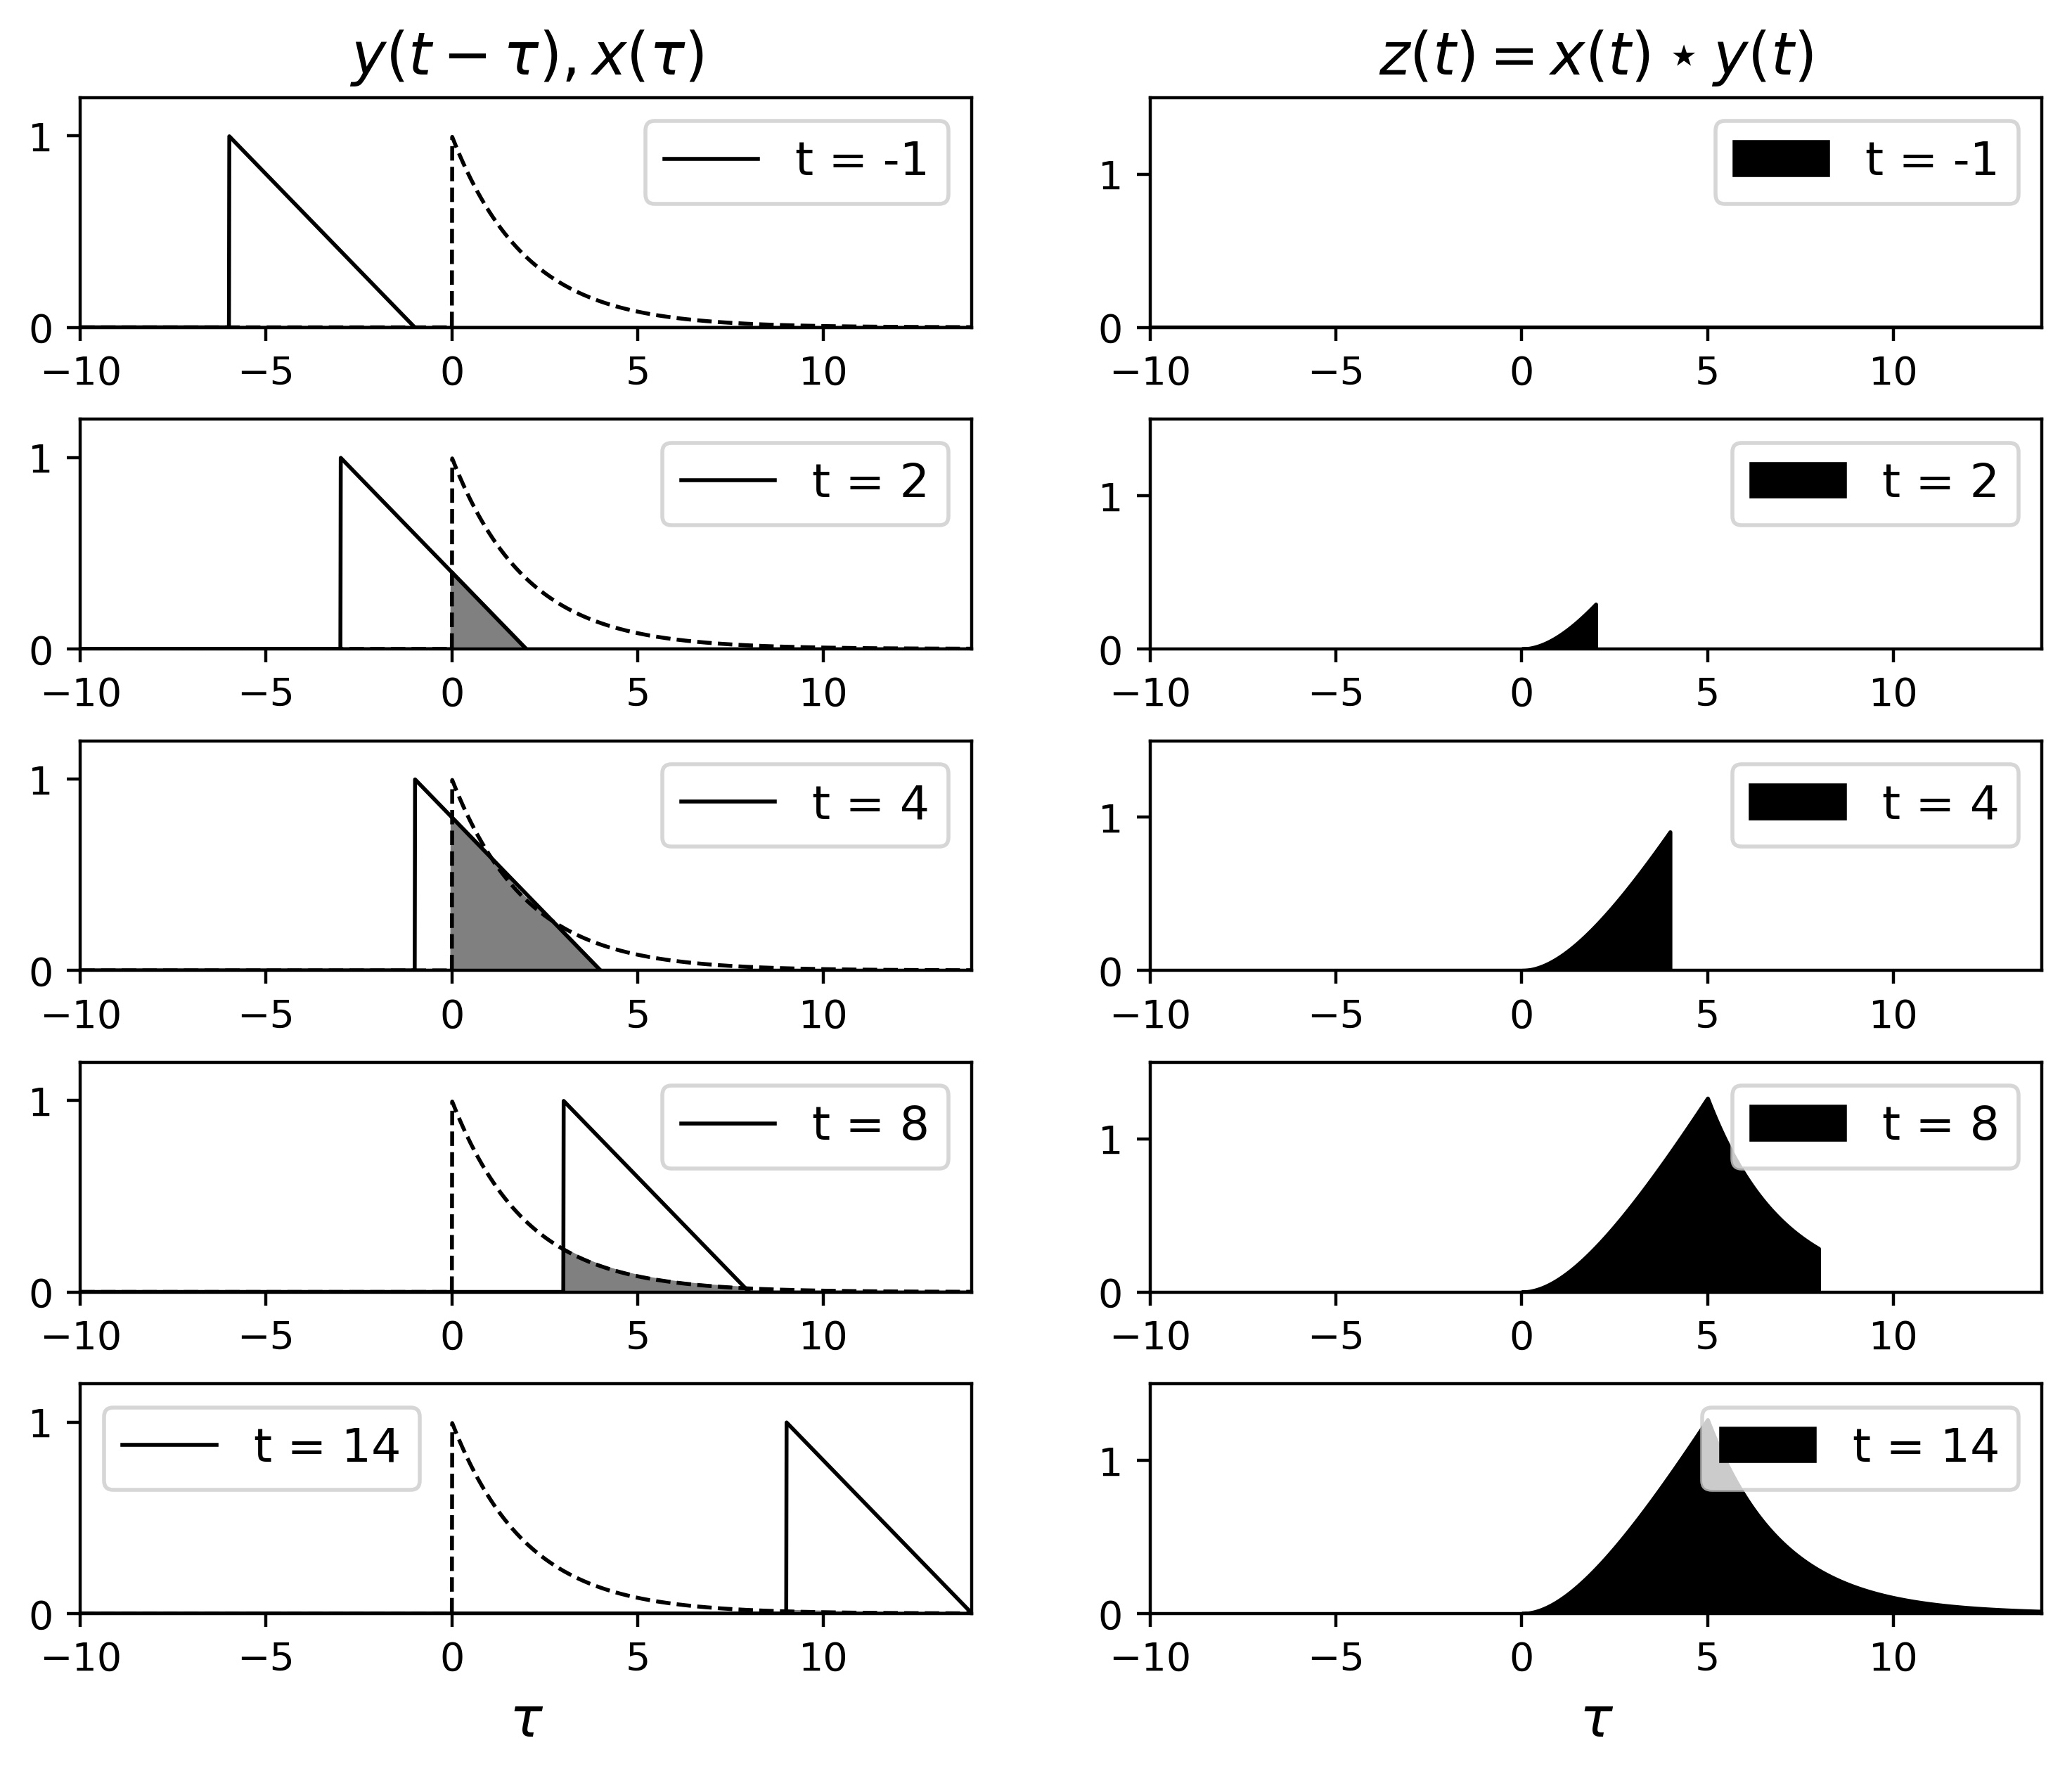
\includegraphics{Figuras/z.jpg}}
	\end{center}
	\vspace{1mm}	% acrescentar o espaçamento vertical apropriado entre a borda inferior da figura e a legenda ou a fonte quando não há legenda (o valor pode ser negativo para subir)
	\legenda{Coluna esquerda: função $y(t - \tau)$ em linha cheia viaja para a direita, passando por $x(\tau)$ em linha tracejada. Coluna direita: resultado da convolução das funções $x(t)$ e $y(t)$. Diferentes valores de $t$ são exibidos.}	% legenda - para deixar sem legenda usar comando \legenda{} (nunca deve-se comentar o comando \legenda)
	\label{fig:2}
	%\FONTE{\url{https://omniweb.gsfc.nasa.gov/form/dx1.html}.}	% fonte consultada (elemento obrigatório, mesmo que seja produção do próprio autor)
\end{figure}

Para sinais discretos, a convolução é assim definida:

\begin{equation}
z[n] = \sum_{k=-\infty}^{\infty} x[k] \ y[n-k],
\end{equation}

onde $k$ e $n$ denotam parâmetros livres que admitem valores inteiros, $x$ e $y$ representam amostras discretas de um sinal, e $x[k]$ é o valor do $k$-ésimo registro do sinal $x$.

\section{Convolução e a transformada de Fourier}

Dada a definição de Transformada de Fourier FT,

\begin{equation}
\text{FT}[x(t)]:: \quad \hat{x}(f) = \int_{-\infty}^{+\infty} x(t) e^{-\imath f t}d t,
\label{eq:ft}
\end{equation}

pode-se mostrar que a transformada de uma convolução é igual ao produto das transformadas individuais:

\begin{equation}
\text{FT}[x \star y] = \text{FT}[x] \cdot \text{FT}[y],
\end{equation}

e esse resultado é conhecido como o \textbf{Teorema da Convolução}. Uma consequência importante desse resultado é:

\begin{equation}
\text{FT}[x \cdot y] = \text{FT}[x] \star \text{FT}[y].
\end{equation}

A Figura \ref{fig:3} ilustra esse Teorema.
\vspace{-10mm}
\begin{figure}[h!]
	\caption{Teorema da Convolução.}
	\vspace{0mm}	% acrescentar o espaçamento vertical apropriado entre o título e a borda superior da figura
	\begin{center}
		\resizebox{13.2cm}{!}{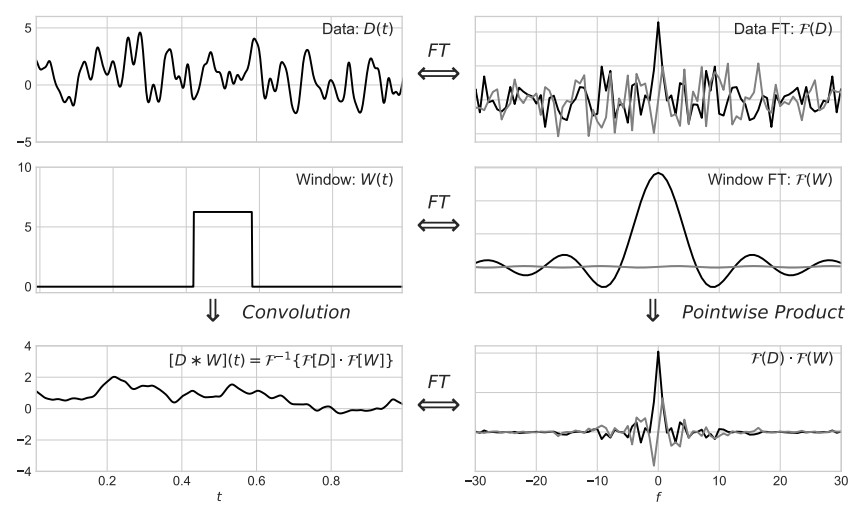
\includegraphics{Figuras/source_t.jpg}}
	\end{center}
	\vspace{1mm}	% acrescentar o espaçamento vertical apropriado entre a borda inferior da figura e a legenda ou a fonte quando não há legenda (o valor pode ser negativo para subir)
	\legenda{Relação entre a convolução de duas funções (coluna esquerda) e o produto ponto a ponto de suas transformadas (coluna da direita). À esquerda as funções estão no domínio do tempo, e à direita estão suas transformadas de Fourier, ou seja, suas representações no domínio da frequência.}	% legenda - para deixar sem legenda usar comando \legenda{} (nunca deve-se comentar o comando \legenda)
	\label{fig:3}
	\vspace{-2mm}
	\FONTE{\citeonline{2017arXiv170309824V}}	% fonte consultada (elemento obrigatório, mesmo que seja produção do próprio autor)
\end{figure}
\vspace{-2mm}
